\documentclass{article}
\usepackage{tikz,amsfonts,amsmath}
\usepackage[paperheight=24in,paperwidth=11in,margin=0.5in]{geometry}
%\usetikzlibrary{shapes.multipart}
\usetikzlibrary{positioning}
\begin{document}
\centering{
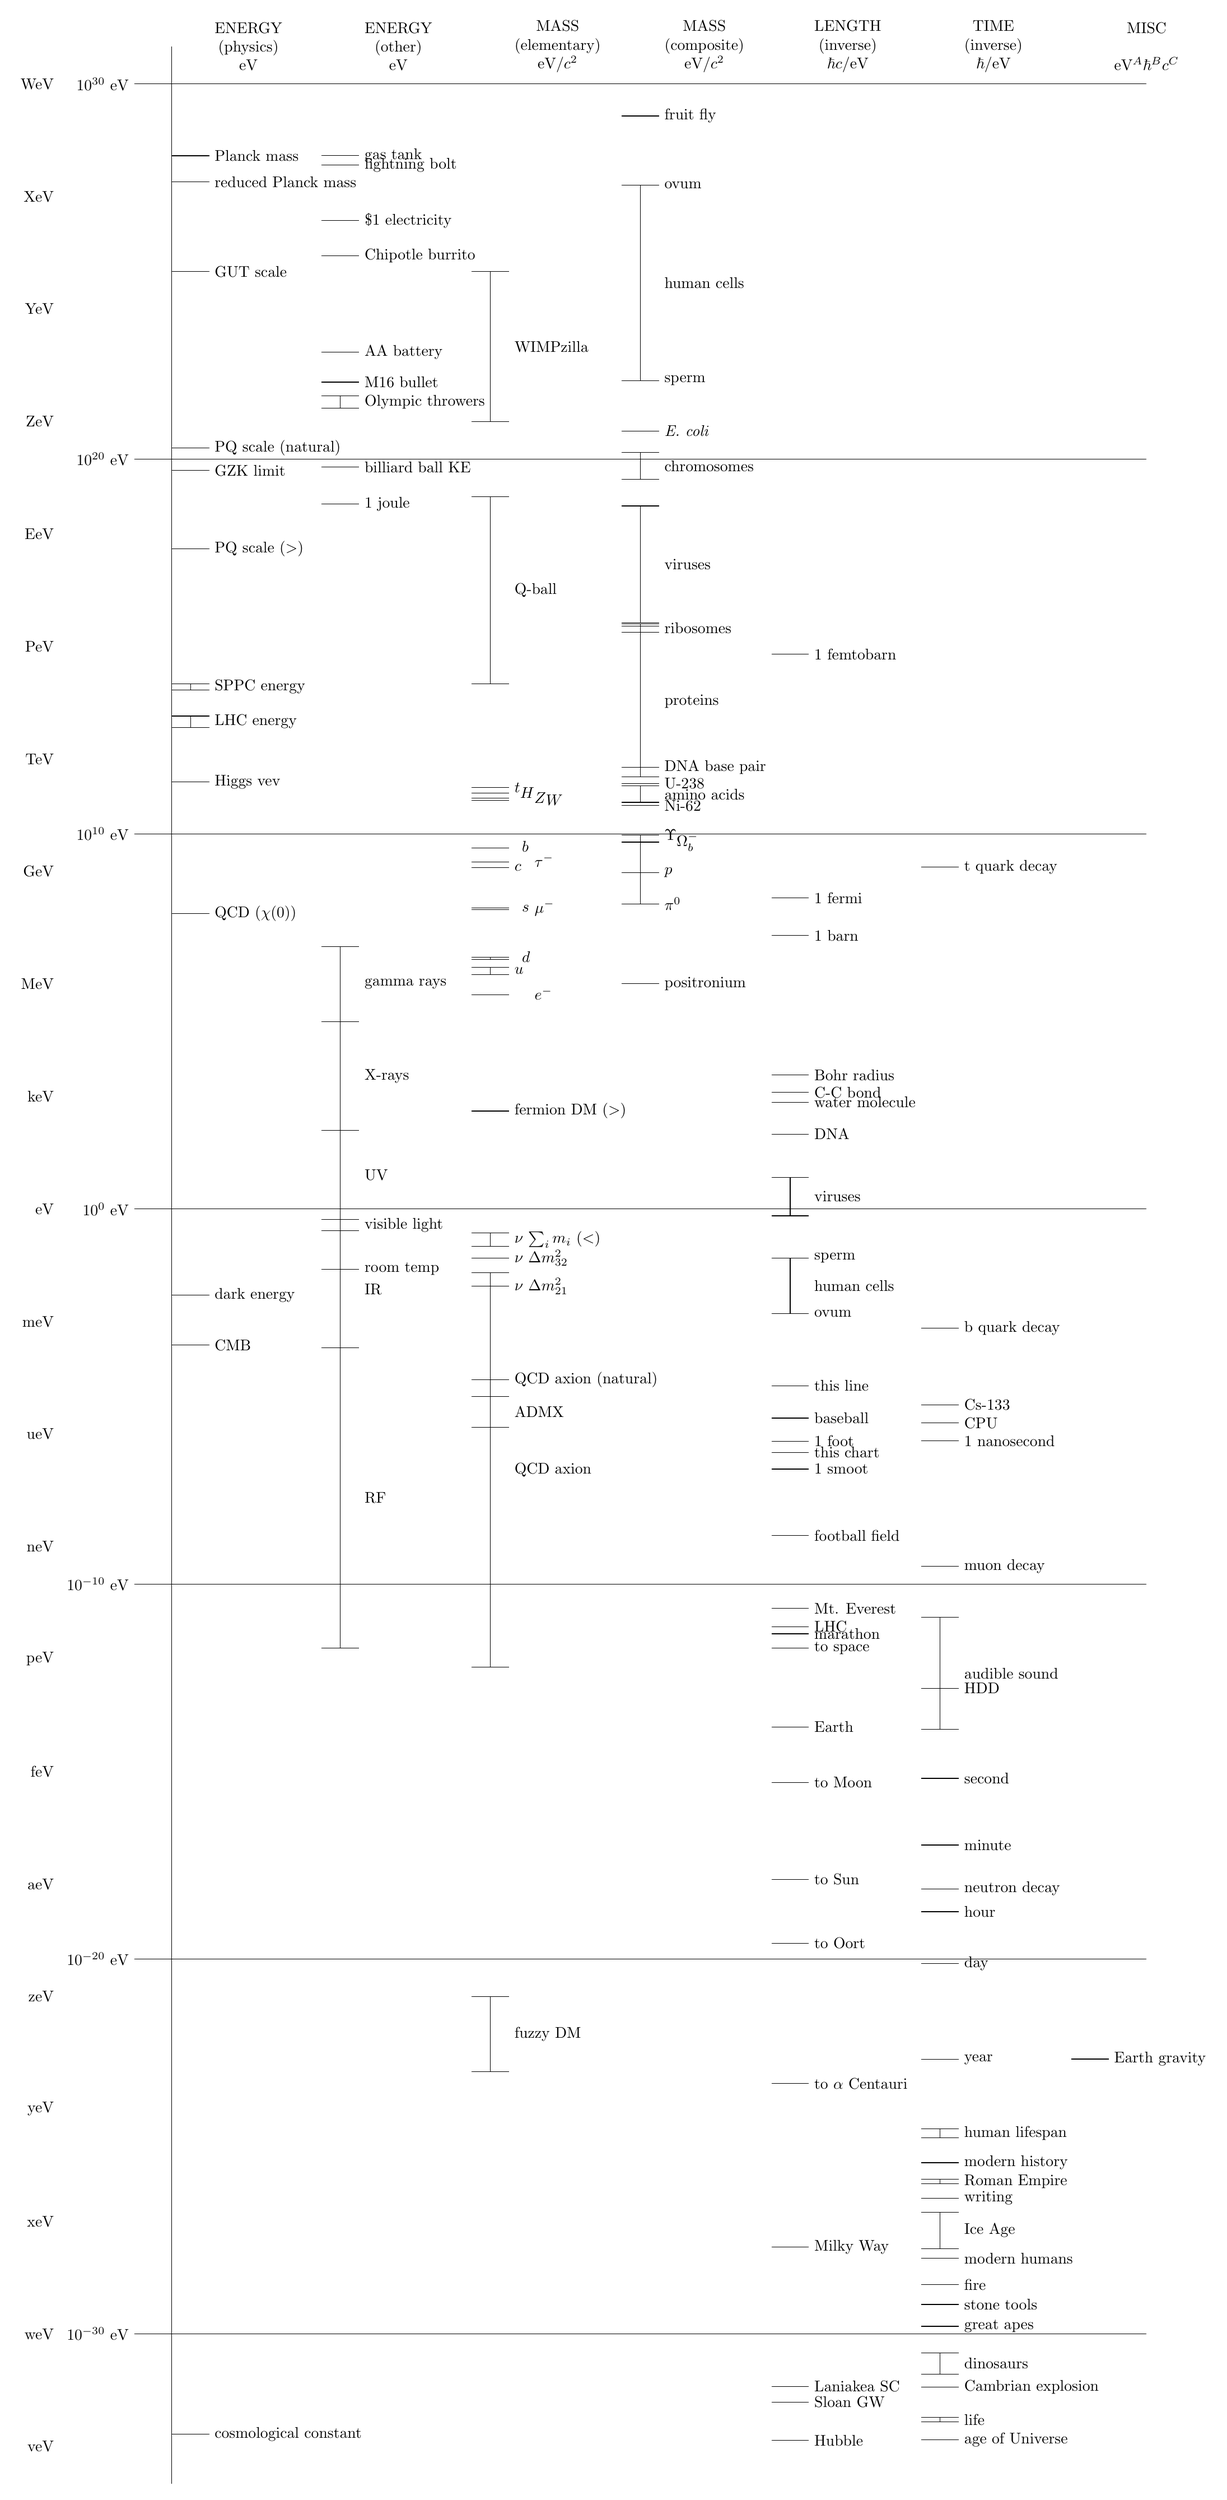
\begin{tikzpicture}[scale=.85,every text node part/.style={align=center}]
\foreach \x in {-30,-20,...,30} {%
  \draw (-1,\x) node[left]{$10^{\x}$ eV}  -- (26,\x) ;
}%
\draw (0, -34) -- (0,31);
\draw (-3,-33) node[left]{veV};
\draw (-3,-30) node[left]{weV};
\draw (-3,-27) node[left]{xeV};
\draw (-3,-24) node[left]{yeV};
\draw (-3,-21) node[left]{zeV};
\draw (-3,-18) node[left]{aeV};
\draw (-3,-15) node[left]{feV};
\draw (-3,-12) node[left]{peV};
\draw (-3,-9) node[left]{neV};
\draw (-3,-6) node[left]{ueV};
\draw (-3,-3) node[left]{meV};
\draw (-3,0) node[left]{ eV};
\draw (-3,3) node[left]{keV};
\draw (-3,6) node[left]{MeV};
\draw (-3,9) node[left]{GeV};
\draw (-3,12) node[left]{TeV};
\draw (-3,15) node[left]{PeV};
\draw (-3,18) node[left]{EeV};
\draw (-3,21) node[left]{ZeV};
\draw (-3,24) node[left]{YeV};
\draw (-3,27) node[left]{XeV};
\draw (-3,30) node[left]{WeV};
\draw (0+1,31) node[right]{ENERGY\\(physics)\\eV};
\draw (0,27.3866) -- (1,27.3866) node[right]{reduced Planck mass};
\draw (0,28.0867) -- (1,28.0867) node[right]{Planck mass};
\draw (0,7.8785) -- (1,7.8785) node[right]{QCD ($\chi(0)$)};
\draw (0,-32.6670) -- (1,-32.6670) node[right]{cosmological constant};
\draw (0,-2.2973) -- (1,-2.2973) node[right]{dark energy};
\draw (0,19.6984) -- (1,19.6984) node[right]{GZK limit};
\draw (0,25.0000) -- (1,25.0000) node[right]{GUT scale};
\draw (0,20.3010) -- (1,20.3010) node[right]{PQ scale (natural)};
\draw (0,17.6021) -- (1,17.6021) node[right]{PQ scale ($>$)};
\draw (0,13.8451) -- (1,13.8451);
\draw (0,14.0000) -- (1,14.0000);
\draw (0.500000,13.8451) -- (0.500000,14.0000);
\draw (1,13.9225) node[right]{SPPC energy};
\draw (0,12.8451) -- (1,12.8451);
\draw (0,13.1461) -- (1,13.1461);
\draw (0.500000,12.8451) -- (0.500000,13.1461);
\draw (1,12.9956) node[right]{LHC energy};
\draw (0,11.3909) -- (1,11.3909) node[right]{Higgs vev};
\draw (0,-3.6295) -- (1,-3.6295) node[right]{CMB};
\draw (4+1,31) node[right]{ENERGY\\(other)\\eV};
\draw (4,28.0963) -- (5,28.0963) node[right]{gas tank};
\draw (4,27.8367) -- (5,27.8367) node[right]{lightning bolt};
\draw (4,26.3635) -- (5,26.3635) node[right]{\$1 electricity};
\draw (4,21.3516) -- (5,21.3516);
\draw (4,21.6874) -- (5,21.6874);
\draw (4.500000,21.3516) -- (4.500000,21.6874);
\draw (5,21.5195) node[right]{Olympic throwers};
\draw (4,22.0506) -- (5,22.0506) node[right]{M16 bullet};
\draw (4,25.4172) -- (5,25.4172) node[right]{Chipotle burrito};
\draw (4,22.8499) -- (5,22.8499) node[right]{AA battery};
\draw (4,19.7865) -- (5,19.7865) node[right]{billiard ball KE};
\draw (4,18.7953) -- (5,18.7953) node[right]{1 joule};
\draw (4,5.0000) -- (5,5.0000);
\draw (4,7.0000) -- (5,7.0000);
\draw (4.500000,5.0000) -- (4.500000,7.0000);
\draw (5,6.0000) node[right]{gamma rays};
\draw (4,2.0934) -- (5,2.0934);
\draw (4,5.0000) -- (5,5.0000);
\draw (4.500000,2.0934) -- (4.500000,5.0000);
\draw (5,3.5467) node[right]{X-rays};
\draw (4,-0.2846) -- (5,-0.2846);
\draw (4,2.0938) -- (5,2.0938);
\draw (4.500000,-0.2846) -- (4.500000,2.0938);
\draw (5,0.9046) node[right]{UV};
\draw (4,-0.2846) -- (5,-0.2846);
\draw (4,-0.5799) -- (5,-0.5799);
\draw (4.500000,-0.2846) -- (4.500000,-0.5799);
\draw (5,-0.4322) node[right]{visible light};
\draw (4,-3.7048) -- (5,-3.7048);
\draw (4,-0.5799) -- (5,-0.5799);
\draw (4.500000,-3.7048) -- (4.500000,-0.5799);
\draw (5,-2.1423) node[right]{IR};
\draw (4,-3.7048) -- (5,-3.7048);
\draw (4,-11.7048) -- (5,-11.7048);
\draw (4.500000,-3.7048) -- (4.500000,-11.7048);
\draw (5,-7.7048) node[right]{RF};
\draw (4,-1.6021) -- (5,-1.6021) node[right]{room temp};
\draw (8+1,31) node[right]{MASS\\(elementary)\\eV$/c^2$};
\draw (8,21.0000) -- (9,21.0000);
\draw (8,25.0000) -- (9,25.0000);
\draw (8.500000,21.0000) -- (8.500000,25.0000);
\draw (9,23.0000) node[right]{WIMPzilla};
\draw (8,14.0000) -- (9,14.0000);
\draw (8,19.0000) -- (9,19.0000);
\draw (8.500000,14.0000) -- (8.500000,19.0000);
\draw (9,16.5000) node[right]{Q-ball};
\draw (8,2.6128) -- (9,2.6128) node[right]{fermion DM ($>$)};
\draw (8,11.2373) -- (9,11.2373) node[right]{$t$};
\draw (8,11.0969) -- (9,11.0969) node[right]{\phantom{$t$}$H$};
\draw (8,10.9590) -- (9,10.9590) node[right]{\phantom{$tH$}$Z$};
\draw (8,10.9031) -- (9,10.9031) node[right]{\phantom{$tHZ$}$W$};
\draw (8,6.2553) -- (9,6.2553);
\draw (8,6.4472) -- (9,6.4472);
\draw (8.500000,6.2553) -- (8.500000,6.4472);
\draw (9,6.3512) node[right]{$u$};
\draw (8,6.6532) -- (9,6.6532);
\draw (8,6.7076) -- (9,6.7076);
\draw (8.500000,6.6532) -- (8.500000,6.7076);
\draw (9,6.6804) node[right]{\phantom{$q$}$d$};
\draw (8,9.1055) -- (9,9.1055) node[right]{$c$};
\draw (8,7.9777) -- (9,7.9777) node[right]{\phantom{$q$}$s$};
\draw (8,9.6212) -- (9,9.6212) node[right]{\phantom{$q$}$b$};
\draw (8,-12.2218) -- (9,-12.2218);
\draw (8,-1.6990) -- (9,-1.6990);
\draw (8.500000,-12.2218) -- (8.500000,-1.6990);
\draw (9,-6.9604) node[right]{QCD axion};
\draw (8,-4.5528) -- (9,-4.5528) node[right]{QCD axion (natural)};
\draw (8,-5.8239) -- (9,-5.8239);
\draw (8,-5.0000) -- (9,-5.0000);
\draw (8.500000,-5.8239) -- (8.500000,-5.0000);
\draw (9,-5.4120) node[right]{ADMX};
\draw (8,-23.0000) -- (9,-23.0000);
\draw (8,-21.0000) -- (9,-21.0000);
\draw (8.500000,-23.0000) -- (8.500000,-21.0000);
\draw (9,-22.0000) node[right]{fuzzy DM};
\draw (8,9.2504) -- (9,9.2504) node[right]{\phantom{$qq$ }$\tau^-$};
\draw (8,8.0253) -- (9,8.0253) node[right]{\phantom{$qq$ }$\mu^-$};
\draw (8,5.7084) -- (9,5.7084) node[right]{\phantom{$qq$ }$e^-$};
\draw (8,-1.0000) -- (9,-1.0000);
\draw (8,-0.6383) -- (9,-0.6383);
\draw (8.500000,-1.0000) -- (8.500000,-0.6383);
\draw (9,-0.8191) node[right]{$\nu$ $\sum_im_i$ ($<$)};
\draw (8,-2.0616) -- (9,-2.0616) node[right]{$\nu$ $\Delta m^2_{21}$};
\draw (8,-1.3063) -- (9,-1.3063) node[right]{$\nu$ $\Delta m^2_{32}$};
\draw (12+1,31) node[right]{MASS\\(composite)\\eV$/c^2$};
\draw (12,29.1469) -- (13,29.1469) node[right]{fruit fly};
\draw (12,27.3052) -- (13,27.3052) node[right]{ovum};
\draw (12,22.0914) -- (13,22.0914);
\draw (12,27.3052) -- (13,27.3052);
\draw (12.500000,22.0914) -- (12.500000,27.3052);
\draw (13,24.6983) node[right]{human cells};
\draw (12,22.0914) -- (13,22.0914) node[right]{sperm};
\draw (12,19.4537) -- (13,19.4537);
\draw (12,20.1751) -- (13,20.1751);
\draw (12.500000,19.4537) -- (12.500000,20.1751);
\draw (13,19.8144) node[right]{chromosomes};
\draw (12,20.7489) -- (13,20.7489) node[right]{\textit{E. coli}};
\draw (12,15.6297) -- (13,15.6297);
\draw (12,18.7489) -- (13,18.7489);
\draw (12.500000,15.6297) -- (12.500000,18.7489);
\draw (13,17.1893) node[right]{viruses};
\draw (12,15.3824) -- (13,15.3824);
\draw (12,15.6002) -- (13,15.6002);
\draw (12.500000,15.3824) -- (12.500000,15.6002);
\draw (13,15.4913) node[right]{ribosomes};
\draw (12,11.5279) -- (13,11.5279);
\draw (12,15.5490) -- (13,15.5490);
\draw (12.500000,11.5279) -- (12.500000,15.5490);
\draw (13,13.5384) node[right]{proteins};
\draw (12,11.7821) -- (13,11.7821) node[right]{DNA base pair};
\draw (12,10.8442) -- (13,10.8442);
\draw (12,11.2788) -- (13,11.2788);
\draw (12.500000,10.8442) -- (12.500000,11.2788);
\draw (13,11.0615) node[right]{amino acids};
\draw (12,10.7616) -- (13,10.7616) node[right]{Ni-62};
\draw (12,11.3458) -- (13,11.3458) node[right]{U-238};
\draw (12,8.1303) -- (13,8.1303) node[right]{$\pi^0$};
\draw (12,9.9759) -- (13,9.9759) node[right]{$\Upsilon$};
\draw (12,8.1303) -- (13,8.1303);
\draw (12,9.9759) -- (13,9.9759);
\draw (12.500000,8.1303) -- (12.500000,9.9759);
\draw (13,9.0531) node[right]{};
\draw (12,8.9722) -- (13,8.9722) node[right]{$p$};
\draw (12,9.7833) -- (13,9.7833) node[right]{\phantom{$\Upsilon$}$\Omega^-_b$};
\draw (12,6.0095) -- (13,6.0095) node[right]{positronium};
\draw (16+1,31) node[right]{LENGTH\\(inverse)\\$\hbar c/$eV};
\draw (16,14.7955) -- (17,14.7955) node[right]{1 femtobarn};
\draw (16,8.2952) -- (17,8.2952) node[right]{1 fermi};
\draw (16,7.2952) -- (17,7.2952) node[right]{1 barn};
\draw (16,3.1077) -- (17,3.1077) node[right]{C-C bond};
\draw (16,3.5709) -- (17,3.5709) node[right]{Bohr radius};
\draw (16,2.8480) -- (17,2.8480) node[right]{water molecule};
\draw (16,1.9942) -- (17,1.9942) node[right]{DNA};
\draw (16,0.8480) -- (17,0.8480);
\draw (16,-0.1819) -- (17,-0.1819);
\draw (16.500000,0.8480) -- (16.500000,-0.1819);
\draw (17,0.3330) node[right]{viruses};
\draw (16,-1.3069) -- (17,-1.3069);
\draw (16,-2.7840) -- (17,-2.7840);
\draw (16.500000,-1.3069) -- (16.500000,-2.7840);
\draw (17,-2.0454) node[right]{human cells};
\draw (16,-1.3069) -- (17,-1.3069) node[right]{sperm};
\draw (16,-2.7840) -- (17,-2.7840) node[right]{ovum};
\draw (16,-4.7117) -- (17,-4.7117) node[right]{this line};
\draw (16,-5.5660) -- (17,-5.5660);
\draw (16,-5.5780) -- (17,-5.5780);
\draw (16.500000,-5.5660) -- (16.500000,-5.5780);
\draw (17,-5.5720) node[right]{baseball};
\draw (16,-6.1888) -- (17,-6.1888) node[right]{1 foot};
\draw (16,-6.4899) -- (17,-6.4899) node[right]{this chart};
\draw (16,-6.9357) -- (17,-6.9357) node[right]{1 smoot};
\draw (16,-8.7048) -- (17,-8.7048) node[right]{football field};
\draw (16,-10.6517) -- (17,-10.6517) node[right]{Mt. Everest};
\draw (16,-11.1362) -- (17,-11.1362) node[right]{LHC};
\draw (16,-11.3281) -- (17,-11.3281) node[right]{marathon};
\draw (16,-11.7048) -- (17,-11.7048) node[right]{to space};
\draw (16,-13.8101) -- (17,-13.8101) node[right]{Earth};
\draw (16,-15.2891) -- (17,-15.2891) node[right]{to Moon};
\draw (16,-17.8797) -- (17,-17.8797) node[right]{to Sun};
\draw (16,-19.5799) -- (17,-19.5799) node[right]{to Oort};
\draw (16,-23.3212) -- (17,-23.3212) node[right]{to $\alpha$ Centauri};
\draw (16,-27.6807) -- (17,-27.6807) node[right]{Milky Way};
\draw (16,-31.3967) -- (17,-31.3967) node[right]{Laniakea SC};
\draw (16,-31.8175) -- (17,-31.8175) node[right]{Sloan GW};
\draw (16,-32.8398) -- (17,-32.8398) node[right]{Hubble};
\draw (20+1,31) node[right]{TIME\\(inverse)\\$\hbar/$eV};
\draw (20,9.1194) -- (21,9.1194) node[right]{t quark decay};
\draw (20,-3.1816) -- (21,-3.1816) node[right]{b quark decay};
\draw (20,-5.2182) -- (21,-5.2182) node[right]{Cs-133};
\draw (20,-5.7045) -- (21,-5.7045) node[right]{CPU};
\draw (20,-6.1816) -- (21,-6.1816) node[right]{1 nanosecond};
\draw (20,-9.5241) -- (21,-9.5241) node[right]{muon decay};
\draw (20,-13.8806) -- (21,-13.8806);
\draw (20,-10.8806) -- (21,-10.8806);
\draw (20.500000,-13.8806) -- (20.500000,-10.8806);
\draw (21,-12.3806) node[right]{audible sound};
\draw (20,-12.7837) -- (21,-12.7837) node[right]{HDD};
\draw (20,-15.1816) -- (21,-15.1816) node[right]{second};
\draw (20,-16.9598) -- (21,-16.9598) node[right]{minute};
\draw (20,-18.7379) -- (21,-18.7379) node[right]{hour};
\draw (20,-20.1181) -- (21,-20.1181) node[right]{day};
\draw (20,-18.1269) -- (21,-18.1269) node[right]{neutron decay};
\draw (20,-22.6807) -- (21,-22.6807) node[right]{year};
\draw (20,-24.5258) -- (21,-24.5258);
\draw (20,-24.7689) -- (21,-24.7689);
\draw (20.500000,-24.5258) -- (20.500000,-24.7689);
\draw (21,-24.6474) node[right]{human lifespan};
\draw (20,-25.4320) -- (21,-25.4320) node[right]{modern history};
\draw (20,-25.8685) -- (21,-25.8685);
\draw (20,-25.9912) -- (21,-25.9912);
\draw (20.500000,-25.8685) -- (20.500000,-25.9912);
\draw (21,-25.9299) node[right]{Roman Empire};
\draw (20,-26.3797) -- (21,-26.3797) node[right]{writing};
\draw (20,-26.7489) -- (21,-26.7489);
\draw (20,-27.7221) -- (21,-27.7221);
\draw (20.500000,-26.7489) -- (20.500000,-27.7221);
\draw (21,-27.2355) node[right]{Ice Age};
\draw (20,-28.6807) -- (21,-28.6807) node[right]{fire};
\draw (20,-27.9818) -- (21,-27.9818) node[right]{modern humans};
\draw (20,-29.2122) -- (21,-29.2122) node[right]{stone tools};
\draw (20,-29.7947) -- (21,-29.7947) node[right]{great apes};
\draw (20,-30.5003) -- (21,-30.5003);
\draw (20,-31.0663) -- (21,-31.0663);
\draw (20.500000,-30.5003) -- (20.500000,-31.0663);
\draw (21,-30.7833) node[right]{dinosaurs};
\draw (20,-31.4139) -- (21,-31.4139) node[right]{Cambrian explosion};
\draw (20,-32.2248) -- (21,-32.2248);
\draw (20,-32.3378) -- (21,-32.3378);
\draw (20.500000,-32.2248) -- (20.500000,-32.3378);
\draw (21,-32.2813) node[right]{life};
\draw (20,-32.8209) -- (21,-32.8209) node[right]{age of Universe};
\draw (24+1,31) node[right]{MISC\\\\eV$^A\hbar^Bc^C$};
\draw (24,-22.6676) -- (25,-22.6676) node[right]{Earth gravity};

\end{tikzpicture}
}

\end{document}
